\newpage
\chapter{Deep relevance matching model}
\label{chap:drmm}

The main paper studied in this work is \cite{drmm}, a deep relevance
matching model (DRMM) to solve ad-hoc retrieval task developed by
Jiafeng Guo et al.

Their approach is a mix of an interaction-focused model and a
representation-focused one.

\section{Architecture}

The DRMM architecture (see figure \ref{fig:drmm_arch}) takes as input a representation of the local interactions between each query-document term pair (called matching histograms).

These histograms inputs are then processed by a feed forward neural network and aggregated with a term gating network, which in turn contributes to weigh each query term with its IDF or its embedding.

Finally, the score aggregation (the dot product in this implementation) produces the matching score of the initial pair (query, document) which is the value that will be used for ranking.

\begin{figure}
  \centering
  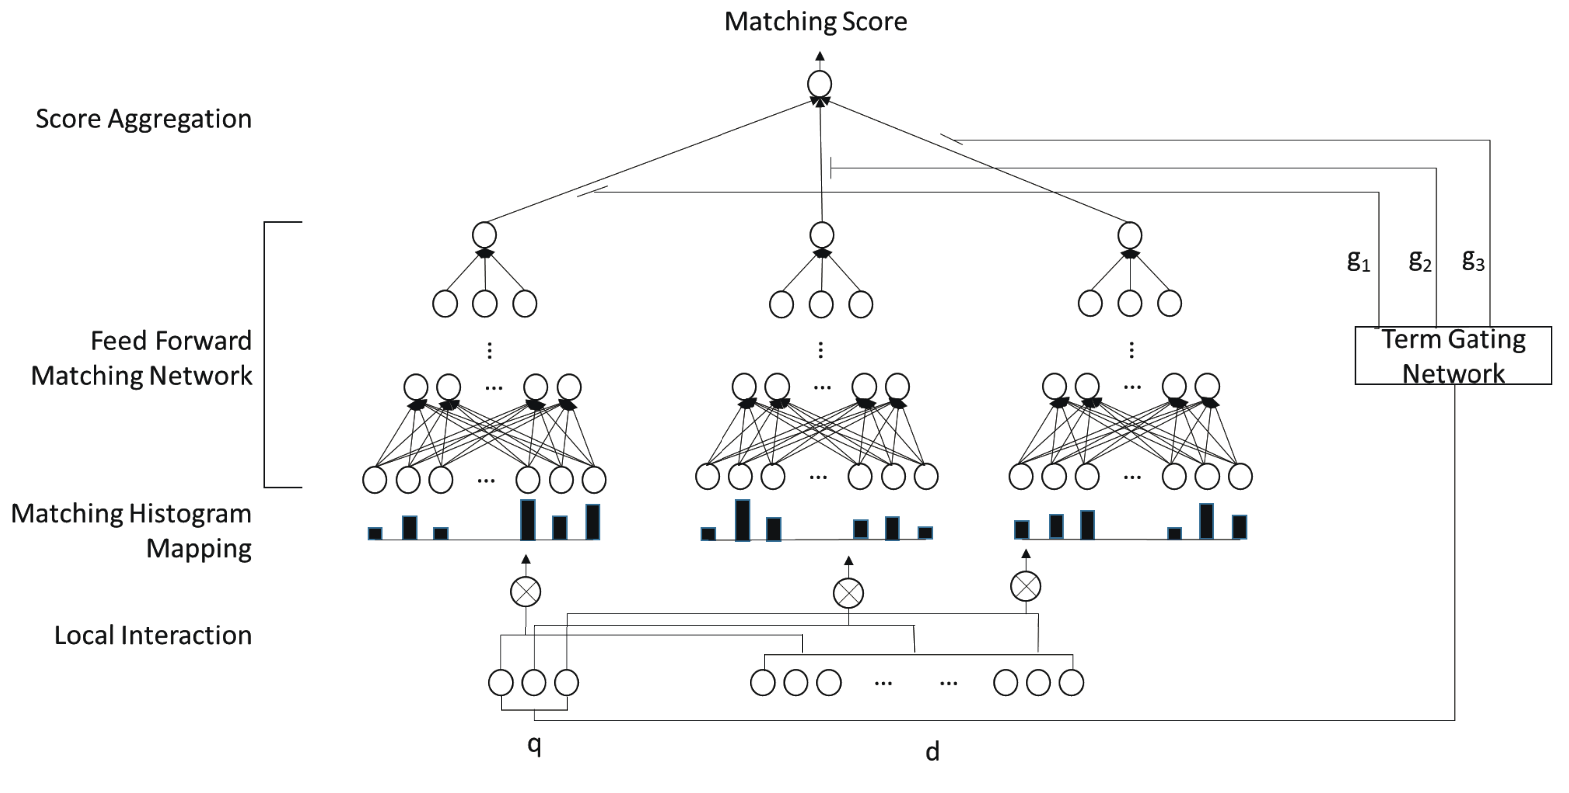
\includegraphics[width=1.0\textwidth]{archDRMM.png}
  \caption{DRMM architecture (reference: \cite{drmm})}
  \label{fig:drmm_arch}
\end{figure}

Each component serves to achieve one of the following three goals:

\begin{itemize}
\item matching histogram mapping is useful to obtain a signature of
both lexical and semantic signals between a query and a document;
\item term gating network takes into account query term importance by weighing them;
\item forward matching network handles diverse matching requirements (i.e. global and local matching).
\end{itemize}

In the next paragraphs each component will be described more in detail.

\subsection{Matching Histogram Mapping}
\label{ssec:mhist}

The inputs of DRMM are the local interactions between each pair of terms
from a query $q$ and a document $d$: $w^{(q)} \otimes w^{(d)} \qquad \forall w^{(q)} \in q, w^{(d)} \in d $ -
where $\otimes$ is the matching function (e.g. cosine similarity).\\

The local interactions represent the matching signals between a (query, document) pair. It is stored into a structure denominated \textit{matching histogram}.\\

An example: let the similarity function be the cosine similarity (so the resulting matching values are in the range [-1, 1]) and let the bin
size be 0.5.

Thus, the bins of the histograms are five: $\{[-1, -0.5), [-0.5, 0),
[0, 0.5), [0.5,1), [1,1]\}$.

Consider the query term ``car'' and the following document sample: (``car'', ``rent'',
``truck'', ``bump'', ``injunction'', ``runway'').

Assume the corresponding cosine similarities: $(1, 0.2, 0.7, 0.3, 0.1)$, then there are three matches in $[0, 0.5)$, one match in $[0.5, 1)$ and one exact match in the last bin.

Thus, the resulting matching histogram is $[0, 0, 3, 1, 1]$.\\

This approach is a strength preserving representation that groups local
interactions according to different levels of signal strengths rather than
their positions.

The main disadvantage of this approach is that all information of word positions in documents is lost.

Guo et al. experimented with three different matching histogram mappings:

\begin{itemize}
\item \textbf{Count-based Histogram (CH)}: the count of local interactions
in each bin is the histogram value, computed as in the previous example (standard version);
\item \textbf{Normalized Histogram (NH)}: the count value in each bin is
normalized by the total count;
\item \textbf{LogCount-based Histogram (LCH)}: logarithm is applied over the
count value in each bin.
\end{itemize}

\section{Semantic matching vs relevance matching}

Matching histogram mapping address both semantic and lexical matching.

Traditional IR models estimate relevance using \textbf{lexical matches} of query terms in document. However, this is not the only choice: representation based models gain evidence of relevance from all document terms based on \textbf{semantic matches} with a query.

Both lexical and semantic matching are important and can be modelled with neural networks.

Guo et al. in \cite{drmm} claim that exact matching of terms is still the most important signal in ad-hoc retrieval, although others (e.g. Huang et al. in \cite{dssm}) consider semantic matching more accurate than lexical matching.

The general intuition is that a good IR model should consider both matches in term space (exact/lexical matches) and semantic matching (matching in the semantic space).

If a term is rare it should be easy to estimate the relevance of a document by individuate patterns of exact matches. On the other hand, if a term is frequent, semantic matching may be more suitable.

\section{Feed forward Matching Network}

Suppose that a query and a document are represented as a set of term vectors denoted by $q = (w_1^{(q)}, w_2^{(q)}, \dots, w_M^{(q)})$
and $d = (w_1^{(d)}, w_2^{(d)}, \dots, w_N^{(d)})$.\\

Let $h$ be the mapping function from local interactions to matching histograms (it can be CH, NH or LCH), $\otimes$ the cosine similarity function and $z_i^{(l)}$ the input of the $l$ layer for the $i$-th query term. The input of the DRMM is denoted by $z_i^{(0)}$:

\begin{equation}
\label{eq:inpFst}
\tag{Input to the first layer of ffnn}
z_i^{(0)} = h(w_i^{(q)} \otimes d) \qquad \forall i = 1 \dots M
\end{equation}

The input to the l-th layer of the feed forward network is:

\begin{equation}
\label{eq:lthdenselayer}
\tag{Input to the l-th layer of ffmn}
z_i^{(l)} = tanh(W^{(l)} \cdot z_i^{(l-1)} + b^{(l)})
\end{equation}

where $W^{(l)}$ denotes the weights matrix and $b^{(l)}$ denotes
the bias term of the l-th layer.

There are three hidden layers of this type for the histogram input and only one layer for the query input, respectively.

Each of them uses the \textit{tanh} as activation function.

\section{Term gating network}

One difference between DRMM and existing interaction-focused models
is that it employs a joint deep architecture at the query term level.

In this way, the model can explicitly model query term importance.

This is achieved by using a term gating network (TGN), which produces an
aggregation weight for each query term controlling how much the
relevance score on that query term contributes to the final relevance value.

The softmax function is employed as the gating function:

\begin{equation}
\label{eq:aggscore}
\tag{Aggregation weight for TGN}
g_i = \frac{exp(w_g \cdot x_i^{(q)})}{\sum_{j=1}^M exp(w_g \cdot x_j^{(q)})} \qquad \forall i = 1 \dots M
\end{equation}

where $w_g$ denotes the weight vector of the term gating network and $x_i^{(q)},
\quad \forall i = 1 \dots M$ denotes the i-th query term input.

The final relevance score for a pair (query, document) is given by the dot product between the output of the term gating network and the feed forward network:

\begin{equation}
\label{eq:drmm_score}
\tag{Relevance score for a pair (q, d)}
s = \sum_{i=1}^{M}g_i \cdot z_i^{(L)}
\end{equation}

There are two variants of the term gating network, depending on its input:

\begin{itemize}
\item \textbf{TV} - the input consists of a term vector.
In this case, $x_i^{(q)}$ (in \ref{eq:aggscore}) corresponds to the i-th query term vector embedding and
$w_g$ is a weight vector with $|w_g| = |x_i^{(q)}|$.
\item \textbf{IDF} - the input consists of the inverse document frequency of
the i-th query term and $w_g$ reduces to a single parameter.
\end{itemize}

\section{Model training}

Since the ad-hoc retrieval task is a ranking problem, Guo et al.
\cite{drmm} employ the \textbf{pairwise hinge loss function} to train their deep relevance matching model.

Given a triple $(q, d^+, d^-)$ where document $d^+$ is ranked higher above
document $d^-$ with respect to query $q$, the loss function is defined as follows:

\begin{equation}
\label{eq:hinge}
\tag{Hinge loss function}
\mathcal{L} (q, d^+, d^-; \Theta) = max(0, 1 - s(q, d^+) + s(q, d^-))
\end{equation}

where $s(q,d)$ denotes the predicted score for $(q,d)$ and $\Theta$ denotes the parameters of the whole model. The equality holds iff $label(q, d) = \pm 1$.

This function aims to assign an higher score to relevant documents w.r.t. non-relevant documents so that the ranking list produced will have high precision at lower cutoffs.

The training is performed using mini-batches stochastic gradient descent.

Guo et al. \cite{drmm} applied stochastic gradient descent algorithm \textit{Adagrad} with mini-batches (20 in size) but they don't report the initial learning rate (which has probably been determined empirically) nor the number of epochs.

Adagrad is an algorithm for gradient-based optimization that adapts the learning rate to the parameters, performing smaller updates (i.e. low learning rates) for parameters associated with frequently occurring features, and larger updates (i.e. high learning rates) for parameters associated with infrequent features.
For this reason, it is well-suited for dealing with sparse data.

For regularization, Guo et al. \cite{drmm} found that the early stopping strategy worked well for
the model.

\section{Experimental setup}

To conduct the experiments, the authors used the following settings:

\begin{table}[H]
\begin{center}
\begin{tabular}{p{5cm} p{8cm}}
\textbf{Data and platform} & \textbf{Name} \\ \hline
Text collections & Robust04 \cite{rob04} \\
Search engine & Galago \tablefootnote{\url{https://sourceforge.net/p/lemur/wiki/Galago}} \\
Tokenization & White-space tokenization \\
Stemmer & Krovetz stemmer \\
Stopword list & INQUERY stop list \tablefootnote{\url{https://github.com/igorbrigadir/stopwords/blob/master/en/indri.txt}} \\ 
Term Embeddings & 300-dimensional term vectors trained with Word2Vec \cite{w2v} with the CBOW model
(context window size = 10; negative sample = 10; subsampling of frequent words
with sampling threshold of $10^{-4}$). Each corpus was pre-processed by
removing HTML tags and stemming, all the terms that occur less than 10 times in
the corpus were removed \\
Network configuration & 4-layer architecture: one histogram input layer
(30 nodes), 2 hidden layers in the feed forward matching network (5 and 1 nodes
respectively) and one output layer (1 node) \\ \hline
\end{tabular}
\caption{Data and platform of the experiment}
\end{center}
\end{table}

The authors performed 5-fold cross-validation to minimize overfitting on the small experimental collection: topics for each collection were randomly
divided into five folds; the parameters for each model were tuned on four of five folds and the overall process was repeated five times.

Each evaluation statistic reported by the authors was the average of the five fold-level evaluation values.

The metric to be optimized during training process was MAP.

A \textbf{re-ranking strategy} for efficient computation was adopted: an initial retrieval was performed using Dirichelet Language Model and Bm25 to obtain the top two thousand ranked documents for each topic.

Finally, the top-ranked one thousand documents were compared w.r.t. MAP, normalized discounted cumulative gain at rank twenty (nDCG$@$20), and precision at rank twenty (P$@$20).

The aim is to bring most (hopefully all) relevant documents in the pre-ranked results as high as possible and keep non relevant documents towards the bottom of the run.

The network should be able to generalize to histograms (query/document pair) never seen before (i.e., documents not in the training set).

\section{Observations on the model}

The quality of the relevance judgments is very important: since the moment that documents not presented in the ground truth are considered to be non relevant, if the relevance judgments are incomplete the network may fail to generalize.

Training and validation labels needs to be chosen in a way that prevents overfitting and underfitting, but in the paper there is no mention on how many relevant/non relevant documents should be considered for each topic during a training epoch.

Another question that needs to be addressed is the case of equal input to the model (matching histograms) generated from different pairs (query, document).

To answer this question it is necessary to study the behavior of the function that maps a query/document pair to a histogram.

Such function ($h$ - see equation \ref{eq:inpFst}) needs to be injective in order to generate always different histograms representations: if two different pairs (query, document) have the same matching signals distribution over bins for each query term then they will have the same histogram too.

It turns out that such function is \textit{not} injective, because it only considers matching signals strength.

A trivial case to show this fact is that in which two documents are permutation of each other (since the moment that matching histograms representation does not preserve information about position of words): when they are matched against the same query they produce the same histograms.